\chapter{VRPTW via AI}\label{vrptw-ai}
In this chapter, we will describe our end-to-end deep learning method for solving \gls{vrptw}.

Machine learning and artificial intelligence have been replacing many hand-engineered algorithms and providing state-of-the-art results. In recent years, reinforcement learning \ref{rl} and advances in attention models \ref{attention} has shown great promise to disrupt the field of heuristics algorithms \cite{rl-constraint-opt, attention-route, dpdp}. Heuristics algorithms \cite{heuristics-algo} are incomplete methods that can compute solutions efficiently, but are not able to prove the optimality of a solution. Most of the business challenges do not require the most optimal exact solution \cite{excat-algo} but focus on approximation of the optimal solution in a reasonable time.

\section{Related Work}
Regarding the research of solving the \gls{vrp}, researchers have been mainly concentrating on designing hand-crafted metaheurictis via optimization. However, the great adoption of deep learning is starting to catch up with the field of operations research.

The first relatively successful deep learning model for solving general \gls{vrp} was proposed by Vinyals et al. \cite{vinyals} in the year of 2015 by introducing Pointer Networks. The model uses attention to output
a permutation of the input and the model was trained in the supervised manner by example solutions. In the next year, Bello et al. \cite{actor-critic-pointer} extended the model of Pointer Networks by adopting the Actor-Critic algorithm that introduced \gls{rl} and the model was trained on the training samples and did not require labelled data anymore. The reward function was a simple Euclidean length of the routes. The network showed improved performance on larger instances of 50 nodes over the predecessor model using supervised learning. In 2018, Nazari et al. \cite{nazari} simplified the model of RL-based Pointer Network by omitting the recurrent neural network encoder and replaced it with embedding to D-dimensional vector space. The recurrent neural network is not necessary because the inputs of delivery nodes are not dependent on order \cite{nazari}. There was no deterioration in performance and the model also supported the constraint for solving split delivery \ref{split-delivery}.

In 2018, Kool et al. \cite{attention-route} proposed a new approach and replaced the Pointer Network with Transformers \ref{transformer} using Graph Attention Network \ref{graph-attention-network} instead of positional encoding, and the Actor-Critic algorithm was changed to REINFORCE algorithm. The model showed superior performance. In this thesis, we will extend this model to support the soft time window constraint.

In 2019, Hottung et al. \cite{hottung} introduced a novel approach that was inspired by \gls{lns} \ref{lns} called Neural Large Neighborhood Search. This model learns the destroy and repair operators by using graph attention network and attention mechanism, and it is outperforming the standard metahesuristics on capacitated vehicle routing problem. However, it is still iterative algorithm based on the local search which results in much larger runtime then end-to-end deep learning methods for \gls{vrp}.

In 2021, another paper by Kool et al.\cite{dpdp} was released with a completely new approach. It combines  dynamic programming and deep learning to solve \gls{vrp} and promises much better performance than previous solutions. The method uses deep learning to restrict the dynamic programming search space using a policy derived from graph neural network. In the future, we will explore this method in depth and extend the support of constraints for time windows and pick and deliver problem \ref{pick-and-delivery}

\section{Solution}
The end-to-end deep learning method pro solving \gls{vrptw} is extension of the work done by Kool et al. \cite{attention-route}. 

Let us describe the high-level concept behind the method. Consider we have a model as blackbox which takes \gls{vrptw} instance as an input and outputs probabilities for all the \gls{vrptw} nodes. The probability represents which node should be visited next and by following to the most probable node we get a partial solution which will be considered by the blackbox. We iterate this process until all nodes have been visited and we acquire a feasible plan as shown on Figure \ref{fig:attention-route-diagram}.

    \begin{figure}[ht]
        \centering
        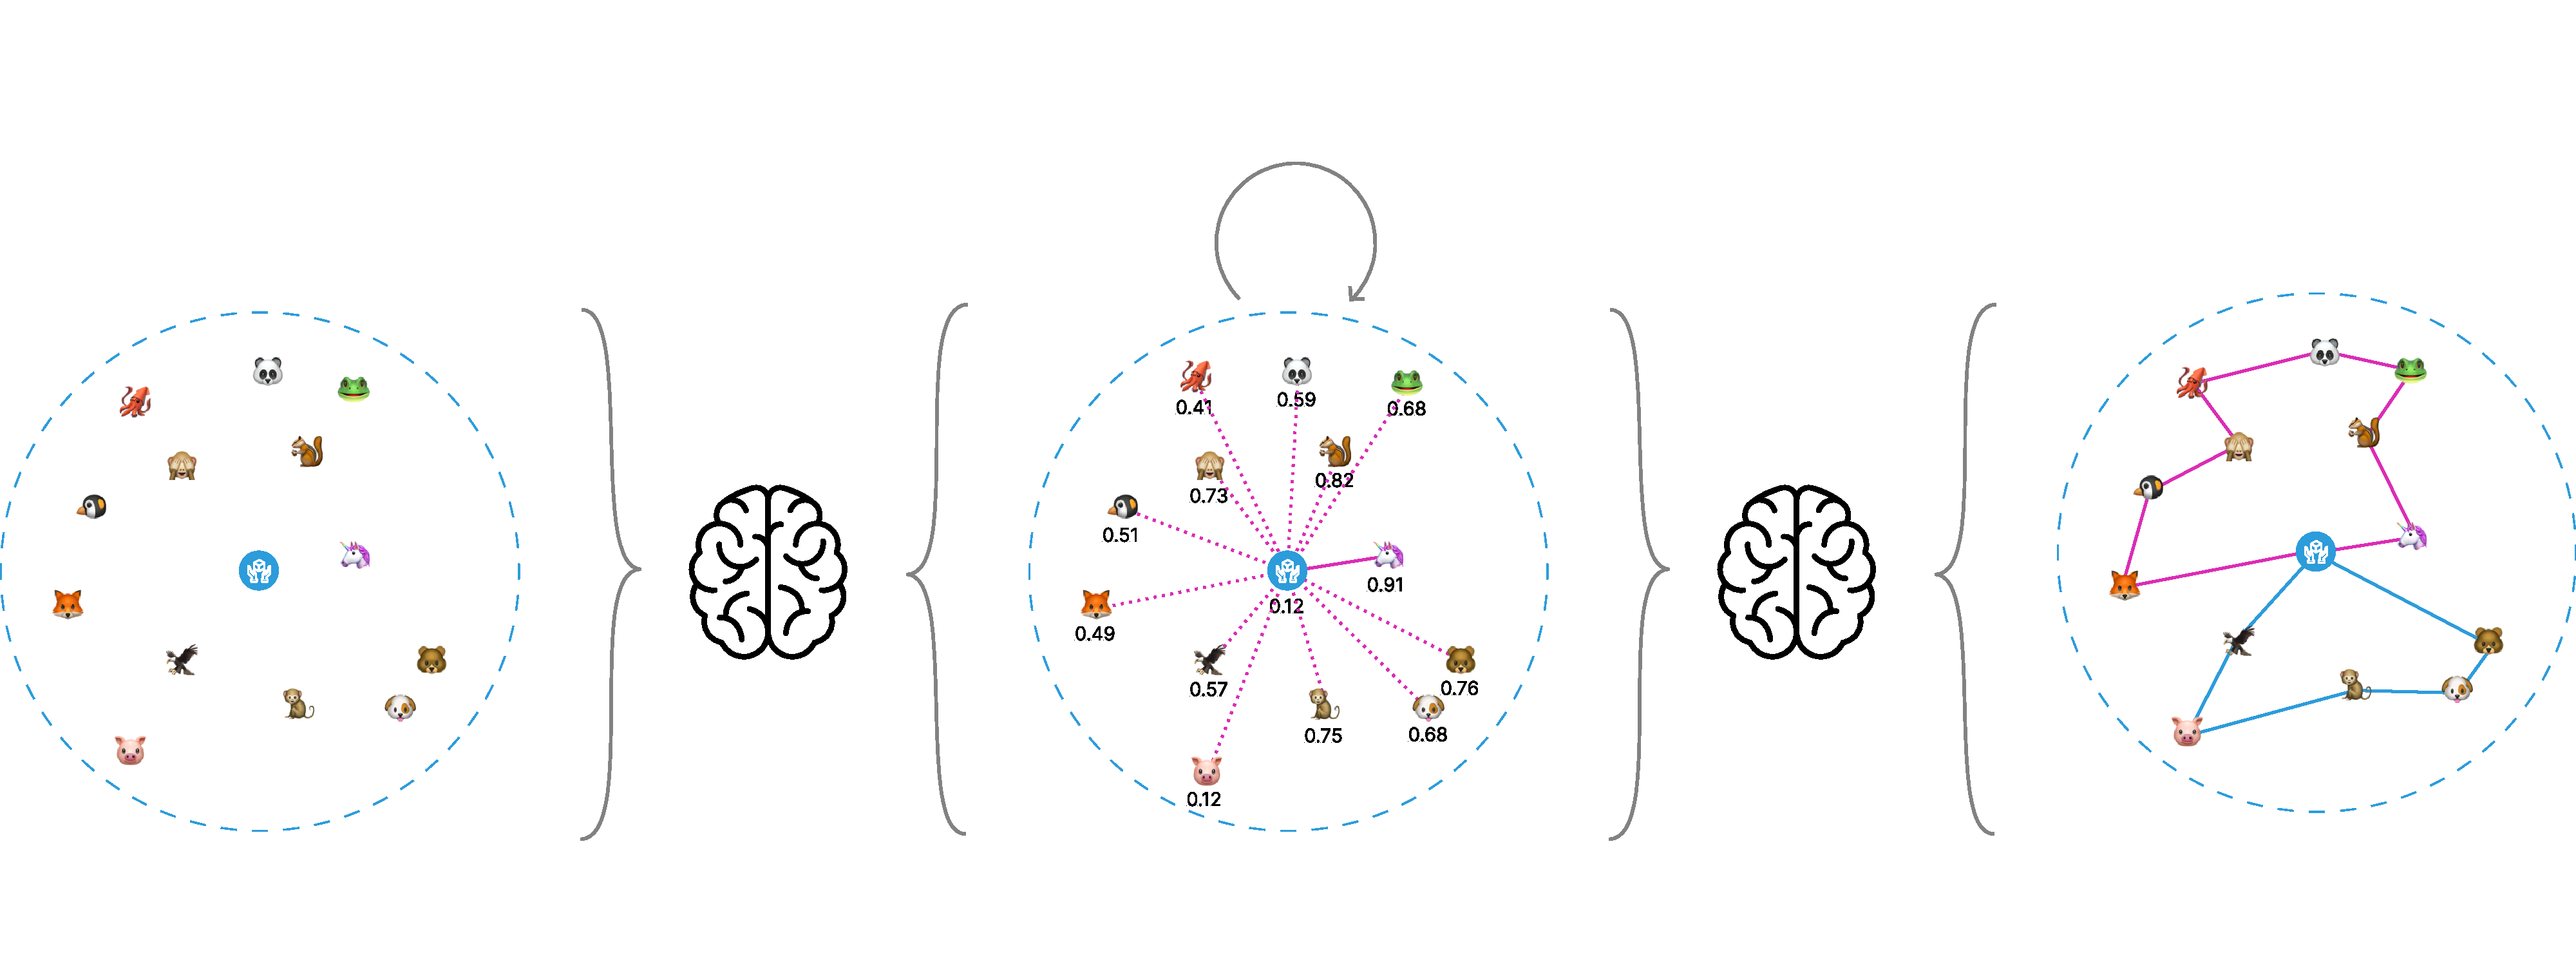
\includegraphics[width=1.0\textwidth]{resources/vrptw-ai/attention-route-diagram.pdf}
        \caption{High-level concept behind the used method.}
        \label{fig:attention-route-diagram}
    \end{figure}

    \subsection{Model Architecture}\label{vrptw-model}
    The model architecture \cite{attention-route} leveraging recent advancements in attention mechanism is here extended by the time window constraint. The model is built upon transformers \ref{transformer}, graph attention network \ref{graph-attention-network}, and reinforcement learning \ref{rl}. The network structure is encoder-decoder that fits well for solving sequential decision problems. The structural input instance is extracted by the encoder \ref{vrptw-encoder} and then the solution is incrementally constructed by the decoder \ref{vrptw-decoder}.
    
    The \gls{vrptw} input instance is consisted from:
    \begin{itemize}\label{input-data}
        \item $X = \{x_1, \cdots, x_n\}$ where $x_i$ is two-dimensional coordinates in the euclidean space.
        \item $x_0$ is the location of depot.
        \item $D = \{d_1, \cdots, d_n\})$ is the demand capacity for each of the locations.
        \item $T = \{(e_1, l_1), \cdots, (e_n, l_n)\})$ is time windows for each of the location where $e_i$ is the beginning and $l_i$ is the end of the considered time window.
    \end{itemize}
    
    The output is the solution of VRPTW instance and is represented as a permutation $\pi$ of locations $X \cup x_0$.
    \begin{itemize}
        \item $\pi = \{\pi_1, \cdots, \pi_T\} \in \{x_0, \cdots, x_n\})$ 
    \end{itemize}
    
    \subsubsection{Encoder}\label{vrptw-encoder}
    The encoder uses graph attention network \ref{graph-attention-network} to embed the node features to graph embedding. Then the decoder architecture is the same as the decoder of transformer \ref{transformer}. Typicaly, the decoder of transformer uses positional encoding \cite{positional-encoding} to embed the input, but in this case it has been replace with \gls{gat} \ref{graph-attention-network} since we deal with graph-based structure and the input order does not matter.
    
    The first step is to perform the initial embedding of input data \ref{input-data} via learned linear projections as in \gls{gat}. The $h_{i}^{l}$ represents the node embedding of layer $l \in \{0, \cdots, N\}$ (N=3).
    \begin{equation}
        \widetilde{x} = \text{concat}(X, D, T)
    \end{equation}
    \begin{equation}
        h_{i}^{0} = \begin{cases} W \widetilde{x}_i + b_i &\mbox{if } i > 0 \\ W \widetilde{x}_0 + b_0 & \mbox{if } n = 0 \end{cases}
    \end{equation}
    
    The node embeddings are updated via $N$ attention layers, each containing multi-head attention \ref{multi-head-attention} (M=8) and a fully connected feed-forward network with normalization. The structure is identical to transformer's encoder \ref{transformer} with additional support of graph structure \ref{graph-attention-network} as shown on Figure \ref{fig:encoder-diagram}.
    
    \begin{figure}[ht]
        \centering
        \includegraphics[width=1.0\textwidth]{resources/vrptw-ai/encoder-diagram.png}
        \caption{Encoder layers \cite{attention-route}}
        \label{fig:encoder-diagram}
    \end{figure}
    
    The equation \ref{encoder-qkv} calculates the query $Q$, key $K$ and value $V$ of multi-head attention layer using the node embeddings and weights $W_m^Q$, $W_m^Q$, and $W_m^Q$, respectively. The number of heads is represented by $m \in \{1, \cdots, M\}$ (M=8).
    
    \begin{equation}\label{encoder-qkv}
        \textbf{q}_{im}^l = W_m^Q h_i^(l-1), \textbf{k}_{im}^l = W_m^K h_i^(l-1), \textbf{v}_{im}^l = W_m^V h_i^(l-1)
    \end{equation}
    
    The query and key values are used in calculating the compatibility $u_{ijm}^l$ of node $i$ with a node $j$ \ref{mha-compatibility}. If node $i$ is not adjecnt to node $j$ then they are not compatible and the value is set to a large negative number.
    
    \begin{equation}\label{mha-compatibility}
        u_{ijm}^l = \begin{cases} q_{im}^l k_{jm}^l &\mbox{if $i$ adjacent to $j$} \\ -\infty &\mbox{otherwise} \end{cases}
    \end{equation}
    
    The attention score $a_{ijm}^l \in [0,1]$ is calculated using softmax from the compatibility values of nodes \ref{encoder-attention-score}
    
    \begin{equation}\label{encoder-attention-score}
        a_{ijm}^l = \dfrac{e^{u_{ijm}^l}}{\sum_{j'=0}^n e^{u_{ij'm}^l}}
    \end{equation}
    
    The transformed $h'_{im}^l$ \ref{h-prime} aggregates all attention scores across neighbour nodes, which is based on GAT \ref{graph-attention-network}. 

    \begin{equation}\label{h-prime}
        h'_{im}^l = \sum_{j=0}^n a_{ijm}^l v_{jm}^l
    \end{equation}
    
    Finally, we may calculate the multi-head attention \ref{transformer} for layer $l$ as a function of $\{h_1^{l-1}, \cdots, h_n^{l-1}\}$ through $h'_{im}^l$.
    
    \begin{equation}
        \text{MHA}_i^l(h_1^{l-1}, \cdots, h_n^{l-1}) = \sum_{m=1}^M W_{m}^O h'_{im}^l
    \end{equation}
    
    \begin{equation}
        \widetilde{h}_i = \text{BN}^l(h_i^{l-1} + \text{MHA}_i^l(h_1^{l-1}, \cdots, h_n^{l-1})))
    \end{equation}    
    \begin{equation}
        h_i^l = \text{BN}^l(\widetilde{h}_i + \text{FF}^l(\widetilde{h}_i))
    \end{equation}
    
    In the final layer, the encoder computes the aggregated embedding of the input graph as the mean of the final node embeddings.
    \begin{equation}
        h^N = \dfrac{1}{n} \sum_{i=1}^m h_i^N
    \end{equation}
    
    The output of the encoder's final layer is passed to the decoder, which is detailed in the next sections \ref{vrptw-decoder}.
    
    \subsubsection{Decoder}\label{vrptw-decoder}
    Decoder works sequentially through timestamps $t \in \{0, \cdots, n\}$, at each timestamp one node is selected to be visited based on partial route $\pi_{1:t-1}$. It is predicting the probability distribution over nodes according to the node embedding and context vector of the encoder \ref{vrptw-encoder}.
    
    \begin{figure}[ht]
        \centering
        \includegraphics[width=1.0\textwidth]{resources/vrptw-ai/decoder-diagram.png}
        \caption{Describes the decoder iteration in the construction of a solution. This diagram very nicely visualizes the process and it was used in the paper by Kool et al. \cite{attention-route}}
        \label{fig:encoder-diagram}
    \end{figure}
    
    The decoder uses a new context vector $h_{c}^{'}$ which represents the state \ref{rl} and it goes as follows:
    \begin{equation}\label{decode-state-vec}
        h_{c}^{'} = \begin{cases} \text{concat}(h_N; h_0^N; D_t) & \mbox{if } t = 0 \\ \text{concat}(h_N; h_{\pi_{1:t-1}}^N; D_t) & \mbox{if } t > 0 \end{cases}
    \end{equation}
    The state of $h_{c}^{'}$ is concatenation of $h_N$, the output of the encoder, $h_{\pi_{1:t-1}}^N$, the embedding of previous partial solution, and $D_t$, the remaining demand capacity of the vehicle.
    
    Due to the fact that the decoder architecture is transformer \ref{transformer}, the next layers are multi-head attentions which are responsible for choosing the next node to visit. This defines the system action \ref{rl}.
    
    The multi-head attention in the decoder is computed in a similar manner as in the decoder \ref{vrptw-encoder} with a little alternation.
    \begin{equation}
        q_{(c)m} = W_m^Q h_{c}^{'}, k_{jm} = W_m^K h_{j}^{N}, v_{jm} = W_m^V h_{j}^{N}
    \end{equation}
    
    \begin{equation}\label{compatibility-decoder}
        u_{(c)j} = \begin{cases} q_c^T k_j &\mbox{if }  d_j <= D_t \text{ and } x_j \notin \pi_{1:t-1} \\ -\infty &\mbox{otherwise} \end{cases}
    \end{equation}
    
    The equation \ref{compatibility-decoder} computes the compatibility score and performs a masking mechanism to mask the nodes which have already been visited during the partial route (besides depot $x_0$) and eliminates nodes where the vehicle capacity would overflow. If we would consider a time window as a hard constraint, the calculation of compatibility would have extended masking mechanism to show only nodes which correspond to the time $t$.
    
    \begin{equation}
        h'_{(c)m} = \sum_{j=0}^n softmax(u_{(c)j}) v_jm
    \end{equation}
        
    \begin{equation}
        h_{c} = \text{MHA}(h_{c}^{'}) = \sum_{m=1}^M W_{m}^O h'_{(c)m}
    \end{equation}
    
    In order to calculate the desired probability $p_{\theta}(\pi_t|X, \pi_{1:t-1})$, a logit layer. The final layer is a single-head attention.
    
    \begin{equation}
        q = W^Q h_c, k_j = W^K h_j^N
    \end{equation}
    
    \begin{equation}
        u_j = \begin{cases} C . \text{tanh}(q^T k_{c}) &\mbox{if }  d_j <= D_t \text{ and } x_j \notin \pi_{1:t-1} \\ -\infty &\mbox{otherwise} \end{cases}
    \end{equation}
    
    \begin{equation}\label{encoder-attention-score}
        p_i = p_{\theta}(\pi_t|X, \pi_{1:t-1}) = \dfrac{e^{u_j}}{\sum_{j'=0}^n e^{u_{j'}}}
    \end{equation}
    
    \subsection{Reinforcement Learning}\label{vrptw-rl}
    The model \ref{vrptw-model} takes \gls{vrptw} instance and outputs probability distribution over nodes $p_{\theta}(\pi|X)$ which is used to sample a full feasible route as a solution $\pi$. The instance of \gls{vrptw} $S$ is defined as concatenation of locations, demand capacity and time windows for each node, $S = [X, D, T]$.
    
    To train the model, we have to define a reward, respectively, a cost function. The model is trained using REINFORCE algorithm \ref{reinforce} as proposed by Kool et al. \cite{attention-route}. The algorithm is based on the computation of the policy gradient, which is defined as
    \begin{equation}\label{encoder-attention-score}
        \nabla_{\theta} \mathcal{L}(\theta|X) = \mathop{\mathbb{E}}[ \mathcal{L}(\pi|X) - b(X)) \nabla \ln \pi (\pi|X))]
    \end{equation}
    
        \subsubsection{VRPTW Cost}\label{vrptw-rl}
        For effectively solving \gls{vrptw}, the cost function is an integral part of a successfully trained model. In this thesis, we propose a new cost function to solve the vehicle routing problem with soft constrained time windows and demand capacity for each node.
        
        The cost function is ranking the given solution of \gls{vrptw} instance. It penalizes the solution based on the length of the routes, early and late visits, and unequal distribution of nodes across vehicles.
        
        For a given \gls{vrptw} instance $S$ and its solution $\pi$, we propose the cost function as follows:
        \newcommand{\norm}[1]{\left\lVert#1\right\rVert}
        \begin{equation}\label{vrptw-cost}
            \mathcal{L}(\pi|S) = dis_p(\pi, S) + t_p(\pi, S) + bal_p(\pi, S)
        \end{equation}
        \begin{equation}\label{distance-cost}
            dis_p(\pi, S) = \sum_{i=0}^N \norm{x_{\pi(i)} - x_{\pi(i+1)}}_2
        \end{equation}
        The equation \ref{distance-cost} calculates the length of all routes in Euclidean space.
        
        \begin{equation}\label{time-cost}
            t_p(\pi, S) = \sum_{i=0}^N (I_{e_i > \widetilde{t}_i} (e_i - \widetilde{t}_i) p_e + I_{l_i < \widetilde{t}_i} (\widetilde{t}_i - l_i) p_l)
        \end{equation}
        The equation \ref{time-cost} calculates the penalty for early or late arrival. The time of the visit for a given node $i$ is defined by vector $\widetilde{t}_i$. We assume that the travel speed is always identical and we approximate that one unit of distance equals to one unit of time. The vector $I$ behaves as a mask $I \in (0, 1)^n$ which represents if either early or late arrival occurred. The penalty for late arrival $p_l$ should be greater than for early arrival $p_e$ and finding the proper penalties will be empirically determined as a part of experiment chapter \ref{penalty-experiment}.
        
        \begin{equation}\label{balance-cost}
            bal_p(\pi, S) = \sigma([|R_0|, \cdots, |R_k|])
        \end{equation}
        The last subpart of the cost function is calculating balance cost \ref{balance-cost} that aims to evenly distribute the number of nodes in a route $R_i$ by minimizing its standard deviation. In logistics, we expect to utilize couriers evenly.
        
        \subsubsection{Training loop}\label{vrptw-loop}
        
        Pseudocode of the \gls{rl} system training loop is as follows
        
        \SetKwInput{KwInput}{Input} 
        \begin{algorithm}[H]
            \KwInput{Number of epoch $E$, steps per epoch $T$, batch size $B$} %significance $\alpha$
            \KwResult{Updated $\theta$ that maximises reward}
            
            Initialize $\theta$ at random\;
            \For{$epoche = 1, 2, \cdots, E$}{
                \For{$steps = 1, 2, \cdots, T$}{
                    Compute context embedding $h^N$ via decoder (\ref{vrptw-encoder});
                    
                    \For{$t = 1, 2, \cdots, N$}{
                        Calculate $p_{\theta}(\pi_t|X, \pi_{1:t-1})$ via encoder for $t$ (\ref{vrptw-decoder});
                        
                        Pick an action based on probability distribution;
                        
                        Update the state by visiting a new node;
                    }
                    
                    Compute reward $\mathcal{L}(\pi|S)$ (\ref{vrptw-cost});
                    
                    %Compute reward baseline;
                    
                    % $\nabla_{\theta} \mathcal{L} \gets \mathop{\mathbb{E}}[ \mathcal{L}(\pi|X) - b(X)) \nabla \ln \pi (\pi|X))]$;
                    
                    $\nabla_{\theta} \mathcal{L} \gets \mathop{\mathbb{E}}[ \mathcal{L}(\pi|X) \nabla \ln \pi (\pi|X))]$;
                    
                    $\theta \gets \text{Adam}(\theta, \nabla_{\theta} \mathcal{L})$;
                }
         }
         \caption{REINFORCE algorithm}
        \end{algorithm}
        
    
    \subsection{Integrating Duration Matrix}
    Real-world application of \gls{vrp} require to obtain the distance and duration matrix which represents the weighted transition between graph nodes. The duration between two locations is typically defined by the infrastructure and speed limits on a given route. Such a duration matrix is calculated using map data such as OpenStreetMap \cite{osm}.
    
    The neural network solving \gls{vrptw} learns to approximate the Euclidean distance between two given points. However, if we would integrate the duration matrix into the cost function of the model, the network would have to derive the duration between two points, which is an impossible task with the given model architecture. Moreover, the planning would be fixed to the location (city) on which the model was trained on.
    
    We propose an indirect integration of the duration matrix for the input instance. We may project the duration matrix into the node locations using multidimensional scaling \cite{mds} which would embed the duration information in a given 2D space.
